\documentclass{fkssolpub}

\usepackage[czech]{babel}
\usepackage{fontspec}
\usepackage{fkssugar}
\usepackage{amsmath}
\usepackage{graphicx}

\author{Ondřej Sedláček}
\school{Gymnázium Oty Pavla} 
\series{2s}
\problem{1} 

\begin{document} 

\begin{figure}[h!]
  \centering
  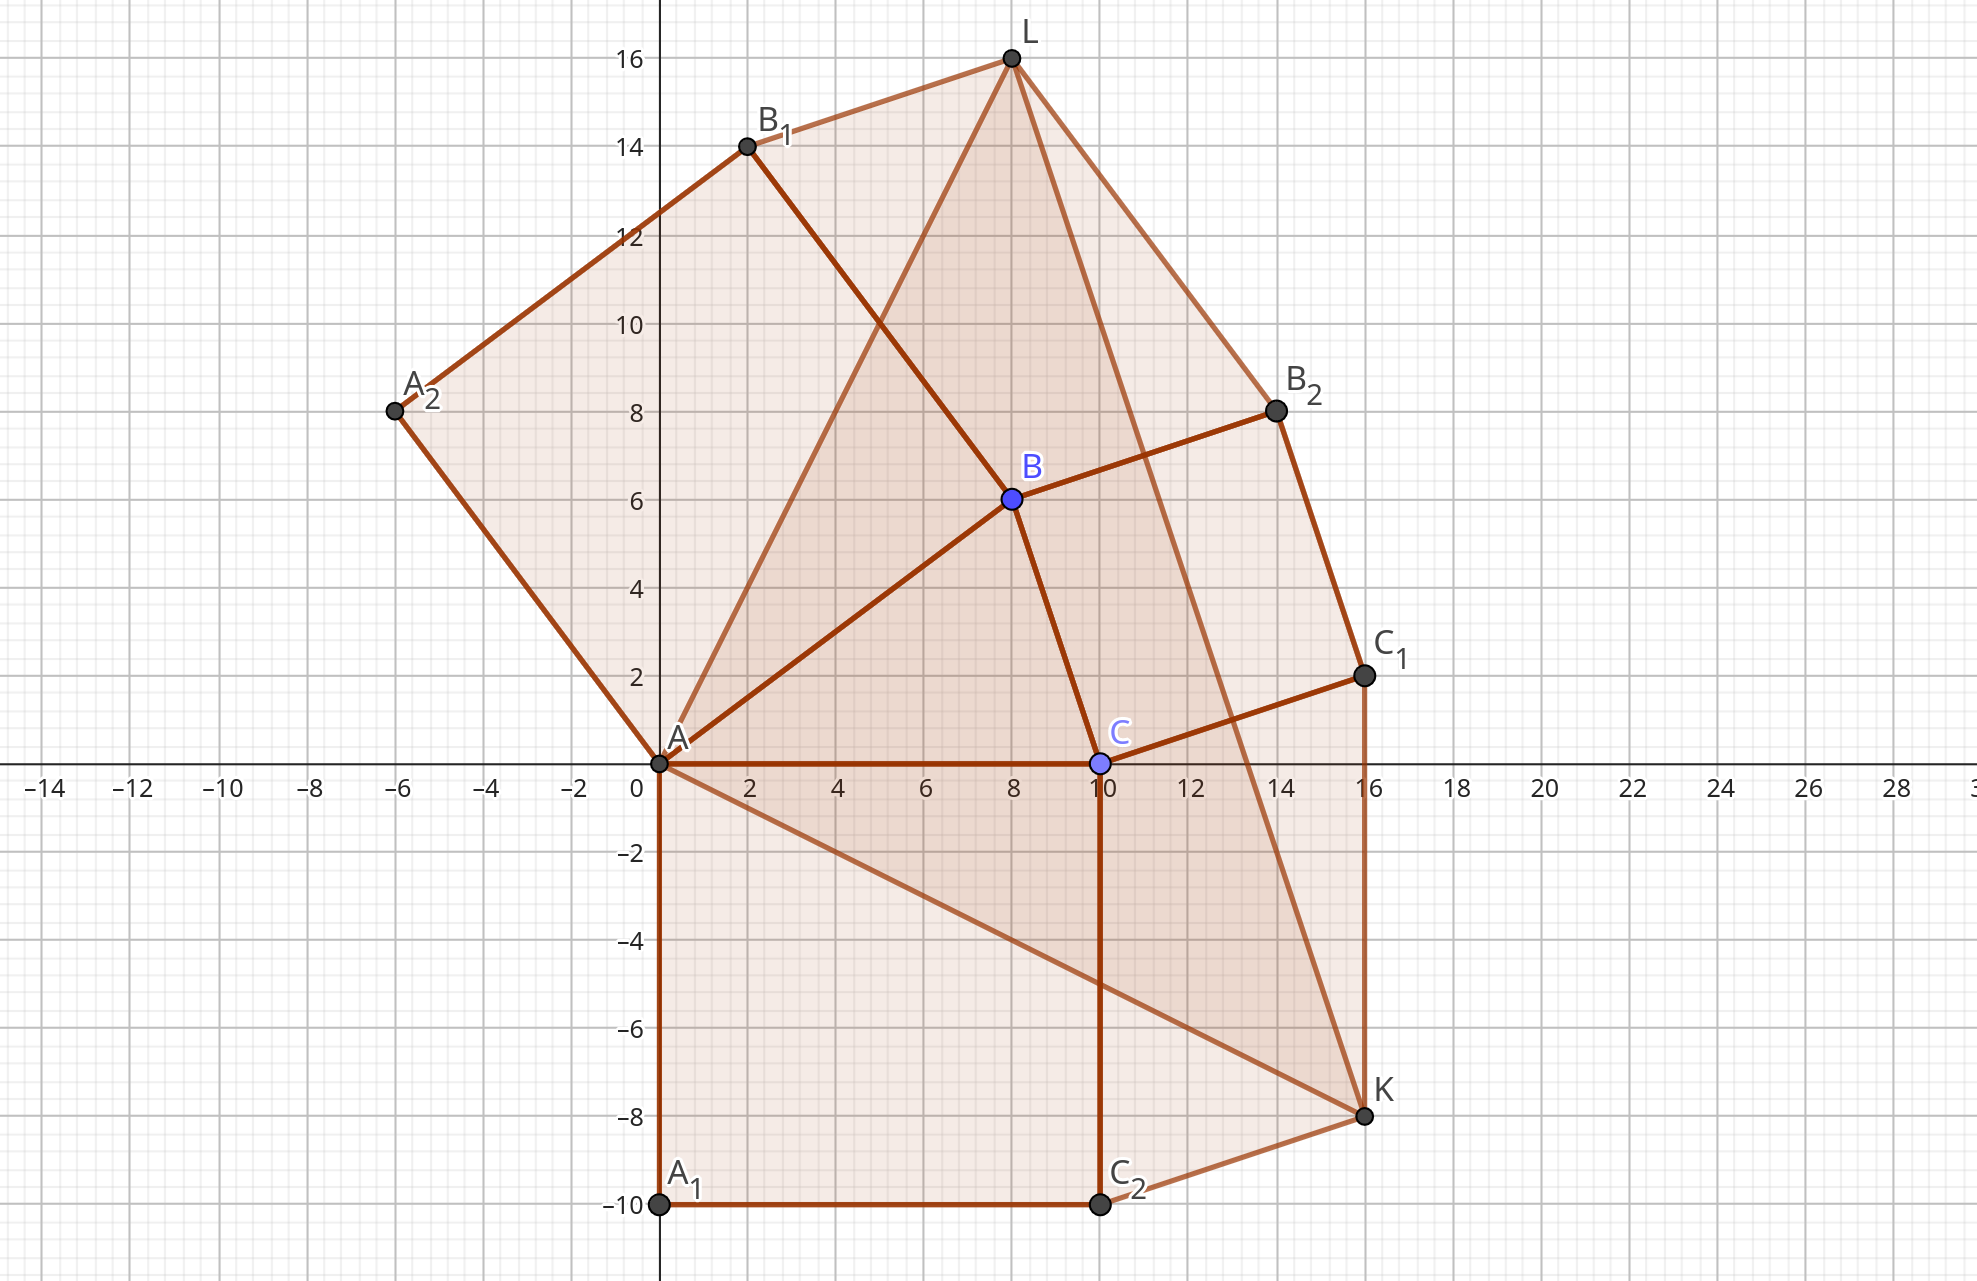
\includegraphics[width=\textwidth]{1-fig.png}
  \label{fig:1}
  \caption{Konstrukce k zpřehlednění popisu}
\end{figure}

Nechť je vrchol $A$ počátek komplexní roviny. Během výpočtu
budu hojně využívat toho, že s body mohu pracovat podobně jako s
vektory, pomocí nichž jsme schopni jednoduše vyjádřit vrcholy
čtverců a rovnoběžníků vůči bodům trojúhelníku. Díky tomu jsme
schopni snadno vyjádřit body $K$ a $L$.

Začněme bodem $K$. Z rovnoběžníku $C_1CC_2K$ víme, že bude platit:

\[
  k = c + (c_1 - c) + (c_2 - c)
\]

Můžeme snadno vypozorovat, že $c_2 - c = a_1 = -ic$ díky zadaným čtvercům.
Druhou stranu rovnoběžníku získáme podobně a bude pro něj platit
$c_1 - c = b - b_2 = i(c - b)$. Tím pádem můžeme bod $K$ vyjádřit jako:

\[
  k = c - ic + i(c - b) = c - ib
\]

Bod $L$ získáme podobným způsobem:

\[
  l = b + (b_1 - b) + (b_2 - b) = b + ib + i(c - b) = b + ic
\]

Aby byl trojúhelník $AKL$ rovnoramenný, musí existovat jednotkové komplexní 
číslo, které je schopno vyjádřit rotaci o úhel $\angle AKL$. Z výrazů,
které nám vyšly, je nápadné, že by to mohly být číslo $i$. A je tomu opravdu
tak:

\[
  ik = i(c - ib) = ic - i^2 b = b + ic = l
\]

Dokázali jsme tedy, že trojúhelník $AKL$ je rovnoramenný a zároveň
pravoúhlý. Tím je tvrzení ze zadání dokázané.

\end{document}
